\section{Analisi SADT}

L'analisi SADT è una tecnica che si avvale di una rappresentazione grafica gerarchica utile per organizzare la progettazione di un generico sistema; per fare ciò si avvale di schede chiamate \textit{attività}.
Si parte dalla definizione del problema generale, quindi si procede con la scomposizione in sottoproblemi in un approccio \textit{top down}; ai livelli inferiori si articola il problema in maniera sempre più dettagliata.
Questo tipo di analisi procede in una scomposizione non temporale ma funzionale del problema; questo approccio ha i ventaggi di una più semplice produzione di documentazione durante la fase di progettazione e una migliore comunicazione tra i diversi componenti del team di progettazione.

I diversi livelli verranno strutturati nel modo seguente:
\begin{itemize}
\item Progettazione del bozzello con gancio;
\item Documentazione dei prodotti esistenti;
\item Scelta delle tipologie di prodotto;
\item Disegno preliminare;
\item Verifica strutturale nominale;
\item Analisi FEA;
\item Disegno della struttura definitiva. 
\end{itemize}

\subsection{Livello A0}
Al primo livello abbiamo l'attività ``Progettazione del bozzello con gancio". Gli input di questo primo livello consistono nei dati di progetto, l'esperienza del progettista, i modelli di progetto e verifica, la documentazione esistente e le normative di riferimento. L'output desiderato consiste nel disegno del progeto; i meccanismi\footnote{Si tratta degli strumenti, fisici o virtuali, di manipolazione dei dati.} sono il progamma CAD utilizzato (SolidWorks) il codice di calcolo agli elementi finiti e il computer.
\begin{figure}[h!]
\centering
  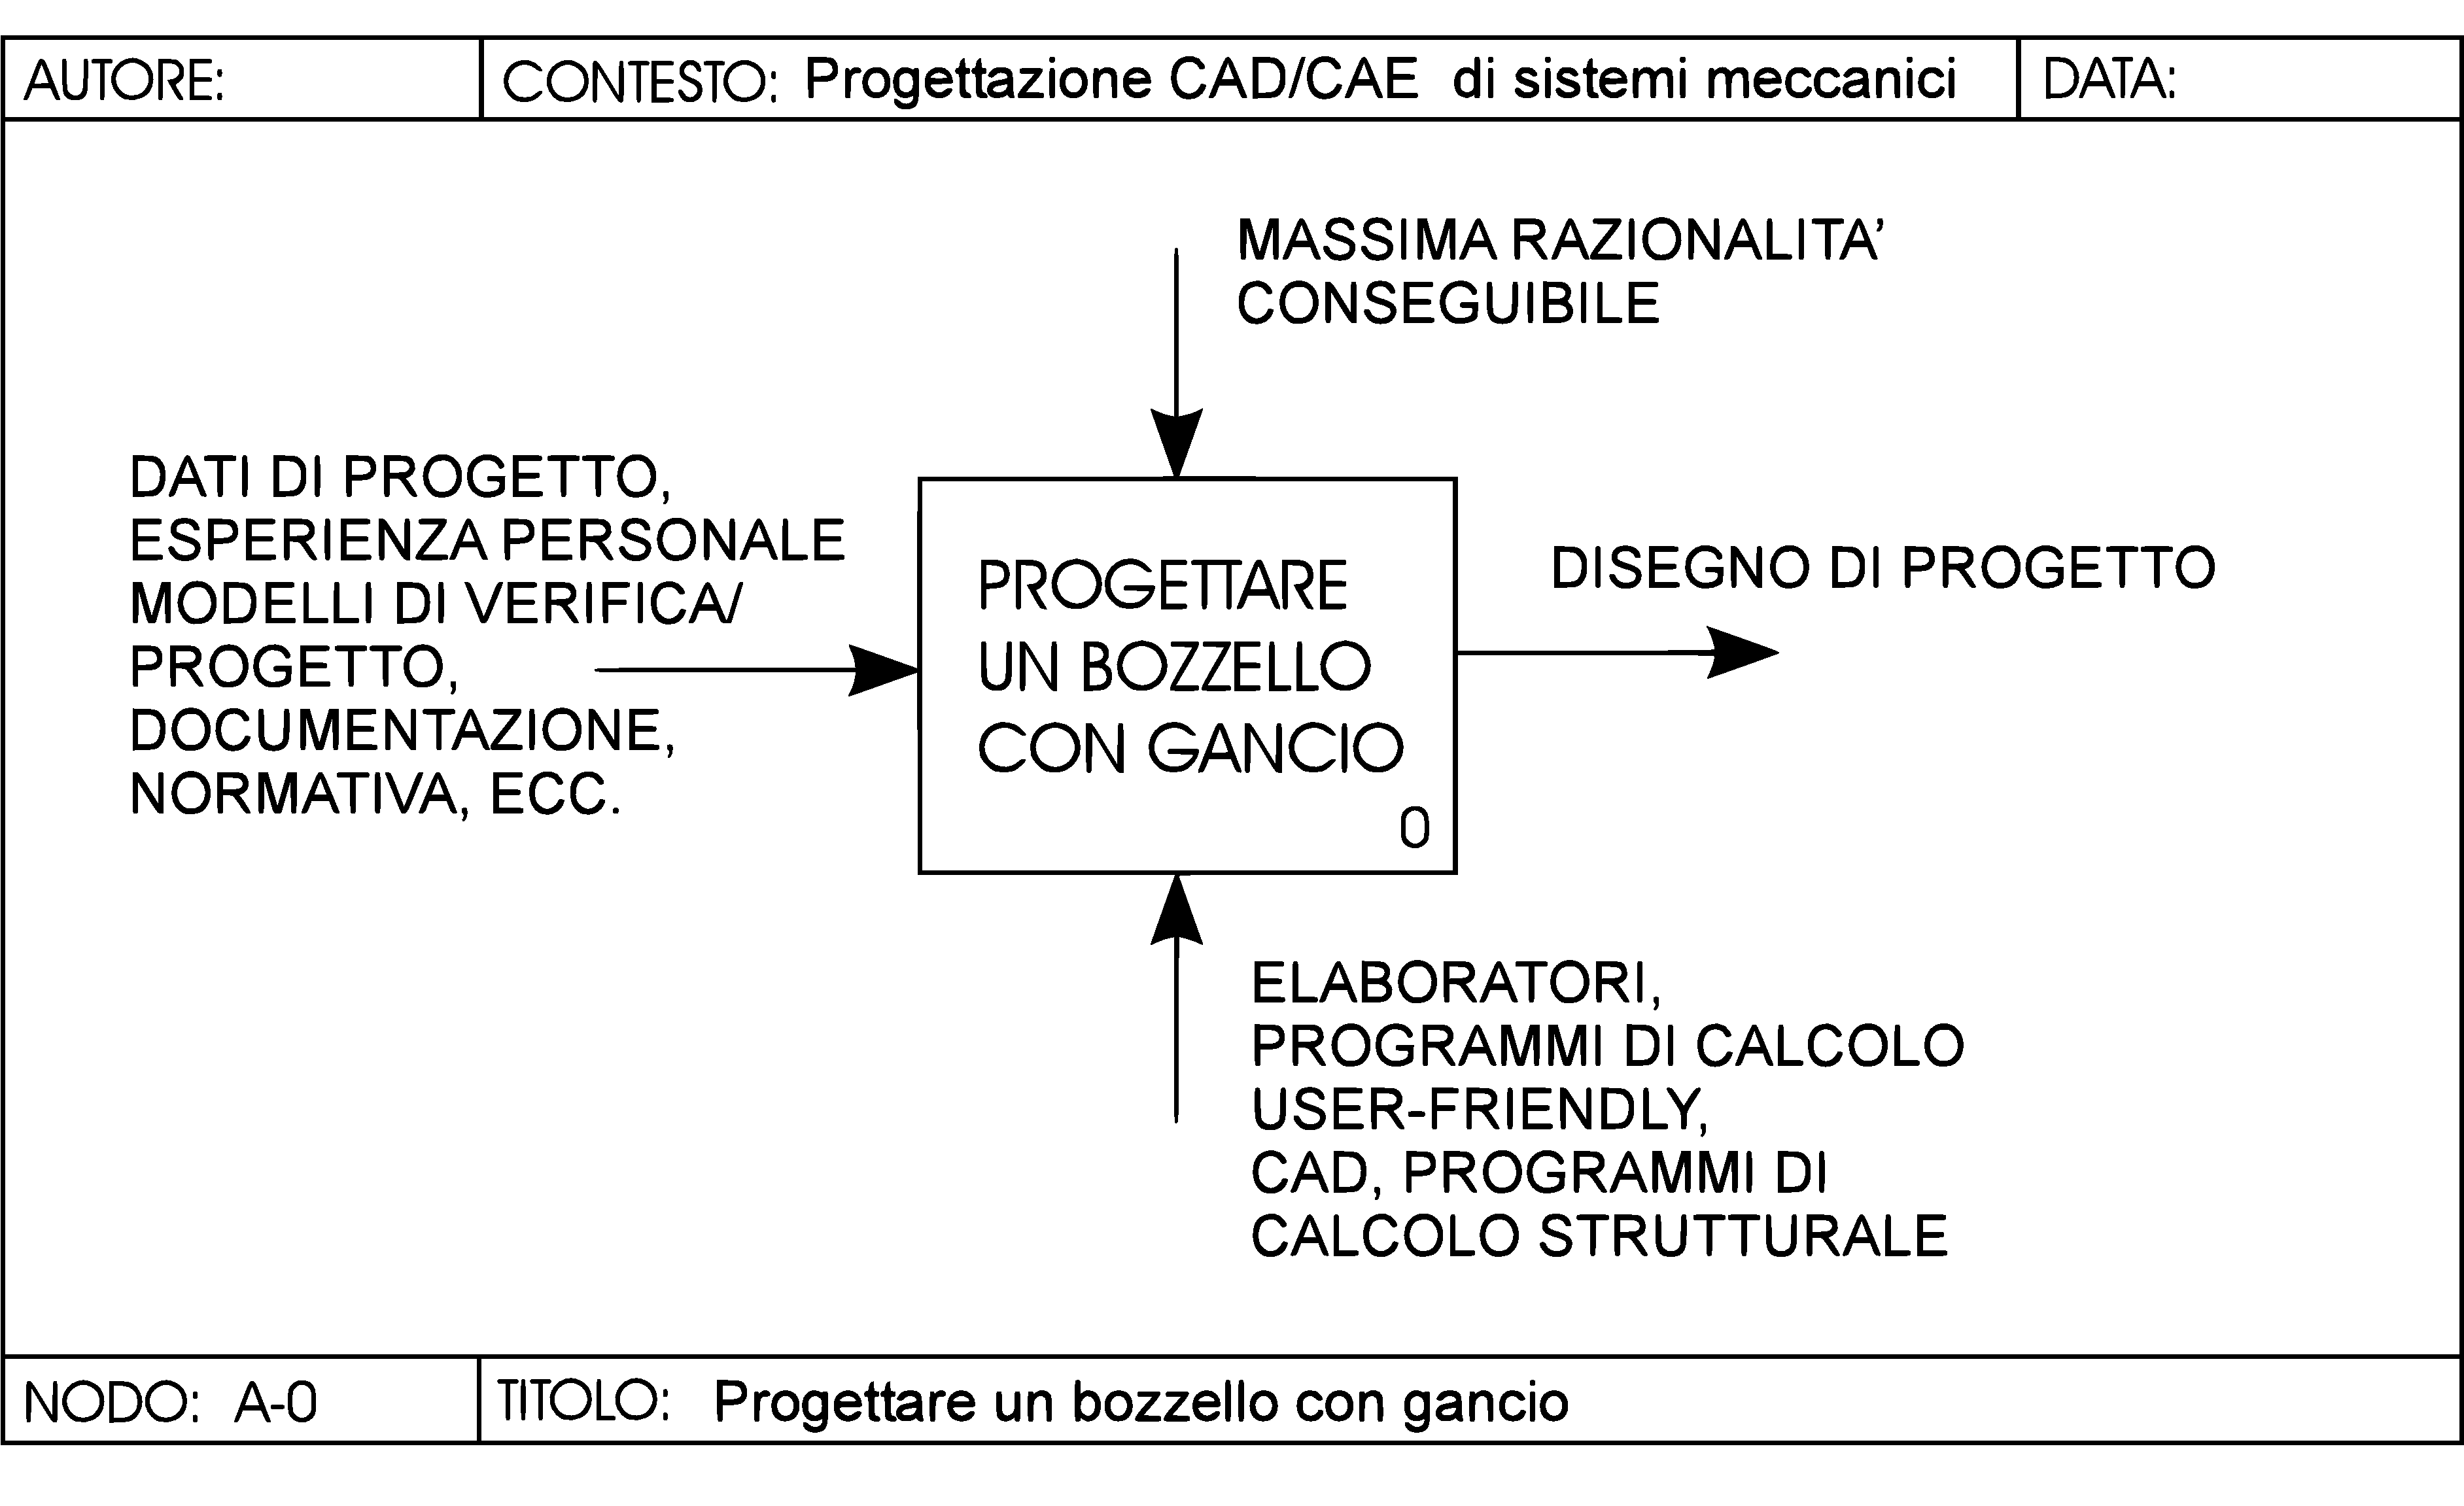
\includegraphics[width=.6\textwidth]{imgs/schedaA0.pdf}
\caption{Nodo A0}
\label{fig:schedaA0}
\end{figure}
I blocchi del diagramma A0 di primo livello individuano le seguenti attività: 
\begin{itemize}
\item Documentare le tipologie esistenti: documentare la produzione nel settore;
\item Scegliere la tipologia adatta: individuare la documentazione tecnica in base alla normativa esistente per i sistemi di sollevamento;
\item Schematizzare il sistema: consista nella stesura di un primo schema strutturale al fine di poter individuare alcune quote di massima ed effettuare le verifiche strutturali nominali;
\item Eseguire la modellazione CAD: a seguito di esito positivo delle verifiche strutturali. In output fornisce il modello solido del bozzello con gancio ed i progetti bidimensionali. 
\item Eseguire le verifiche strutturali FEA: in base alle forze esterne applicate e fissati opportunamente i vincoli, è possibile eseguire un'analisi agli elementi finiti al fine di verificare dal punto di vista strutturale il sistema precedentemente modellato con un grado di precisione superiore ai modelli di scienza delle costruzioni. Se la verifica dovesse avere esito negativo è necessario tornare alla fase di dimensionamento ed effettuare le opportune modifiche. 
\end{itemize}
\begin{figure}[h!]
\centering
  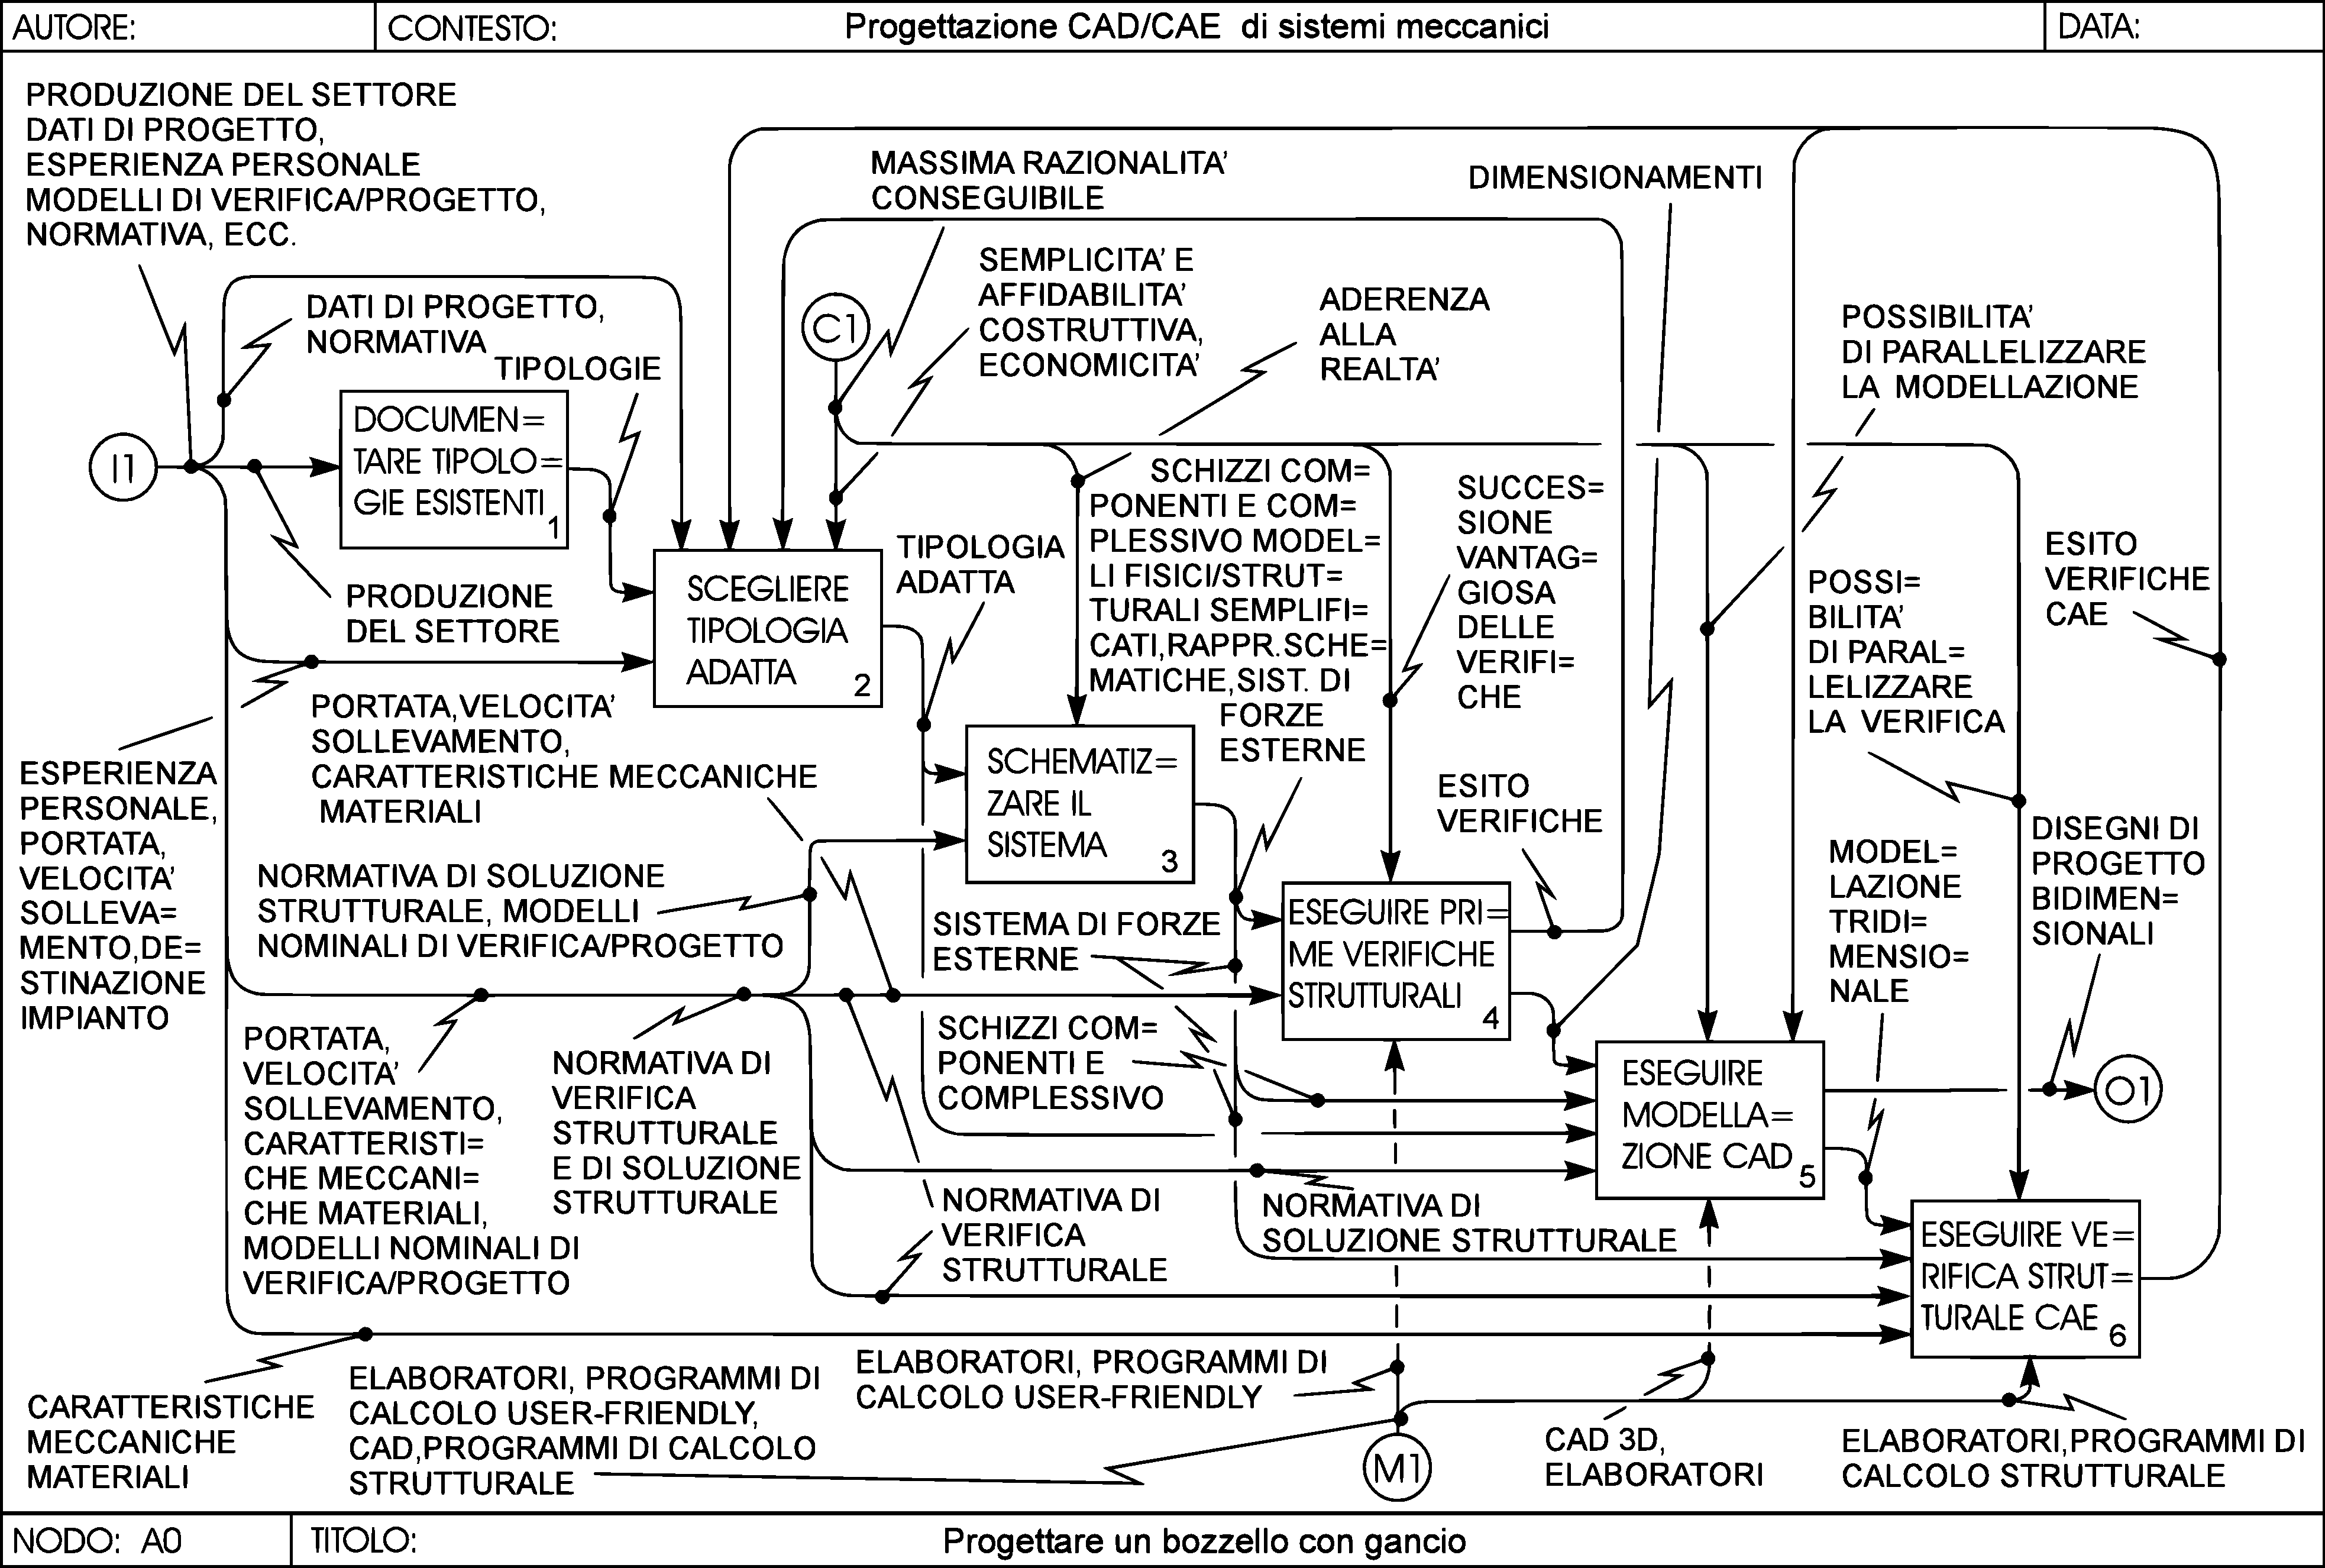
\includegraphics[width=.8\textwidth]{imgs/schedaA0dettaglio.pdf}
\caption{Nodo A0 dettagliato}
\label{fig:schedaA0dettaglio}
\end{figure}

\subsection{Nodo A3}
\begin{figure}[h!]
\centering
  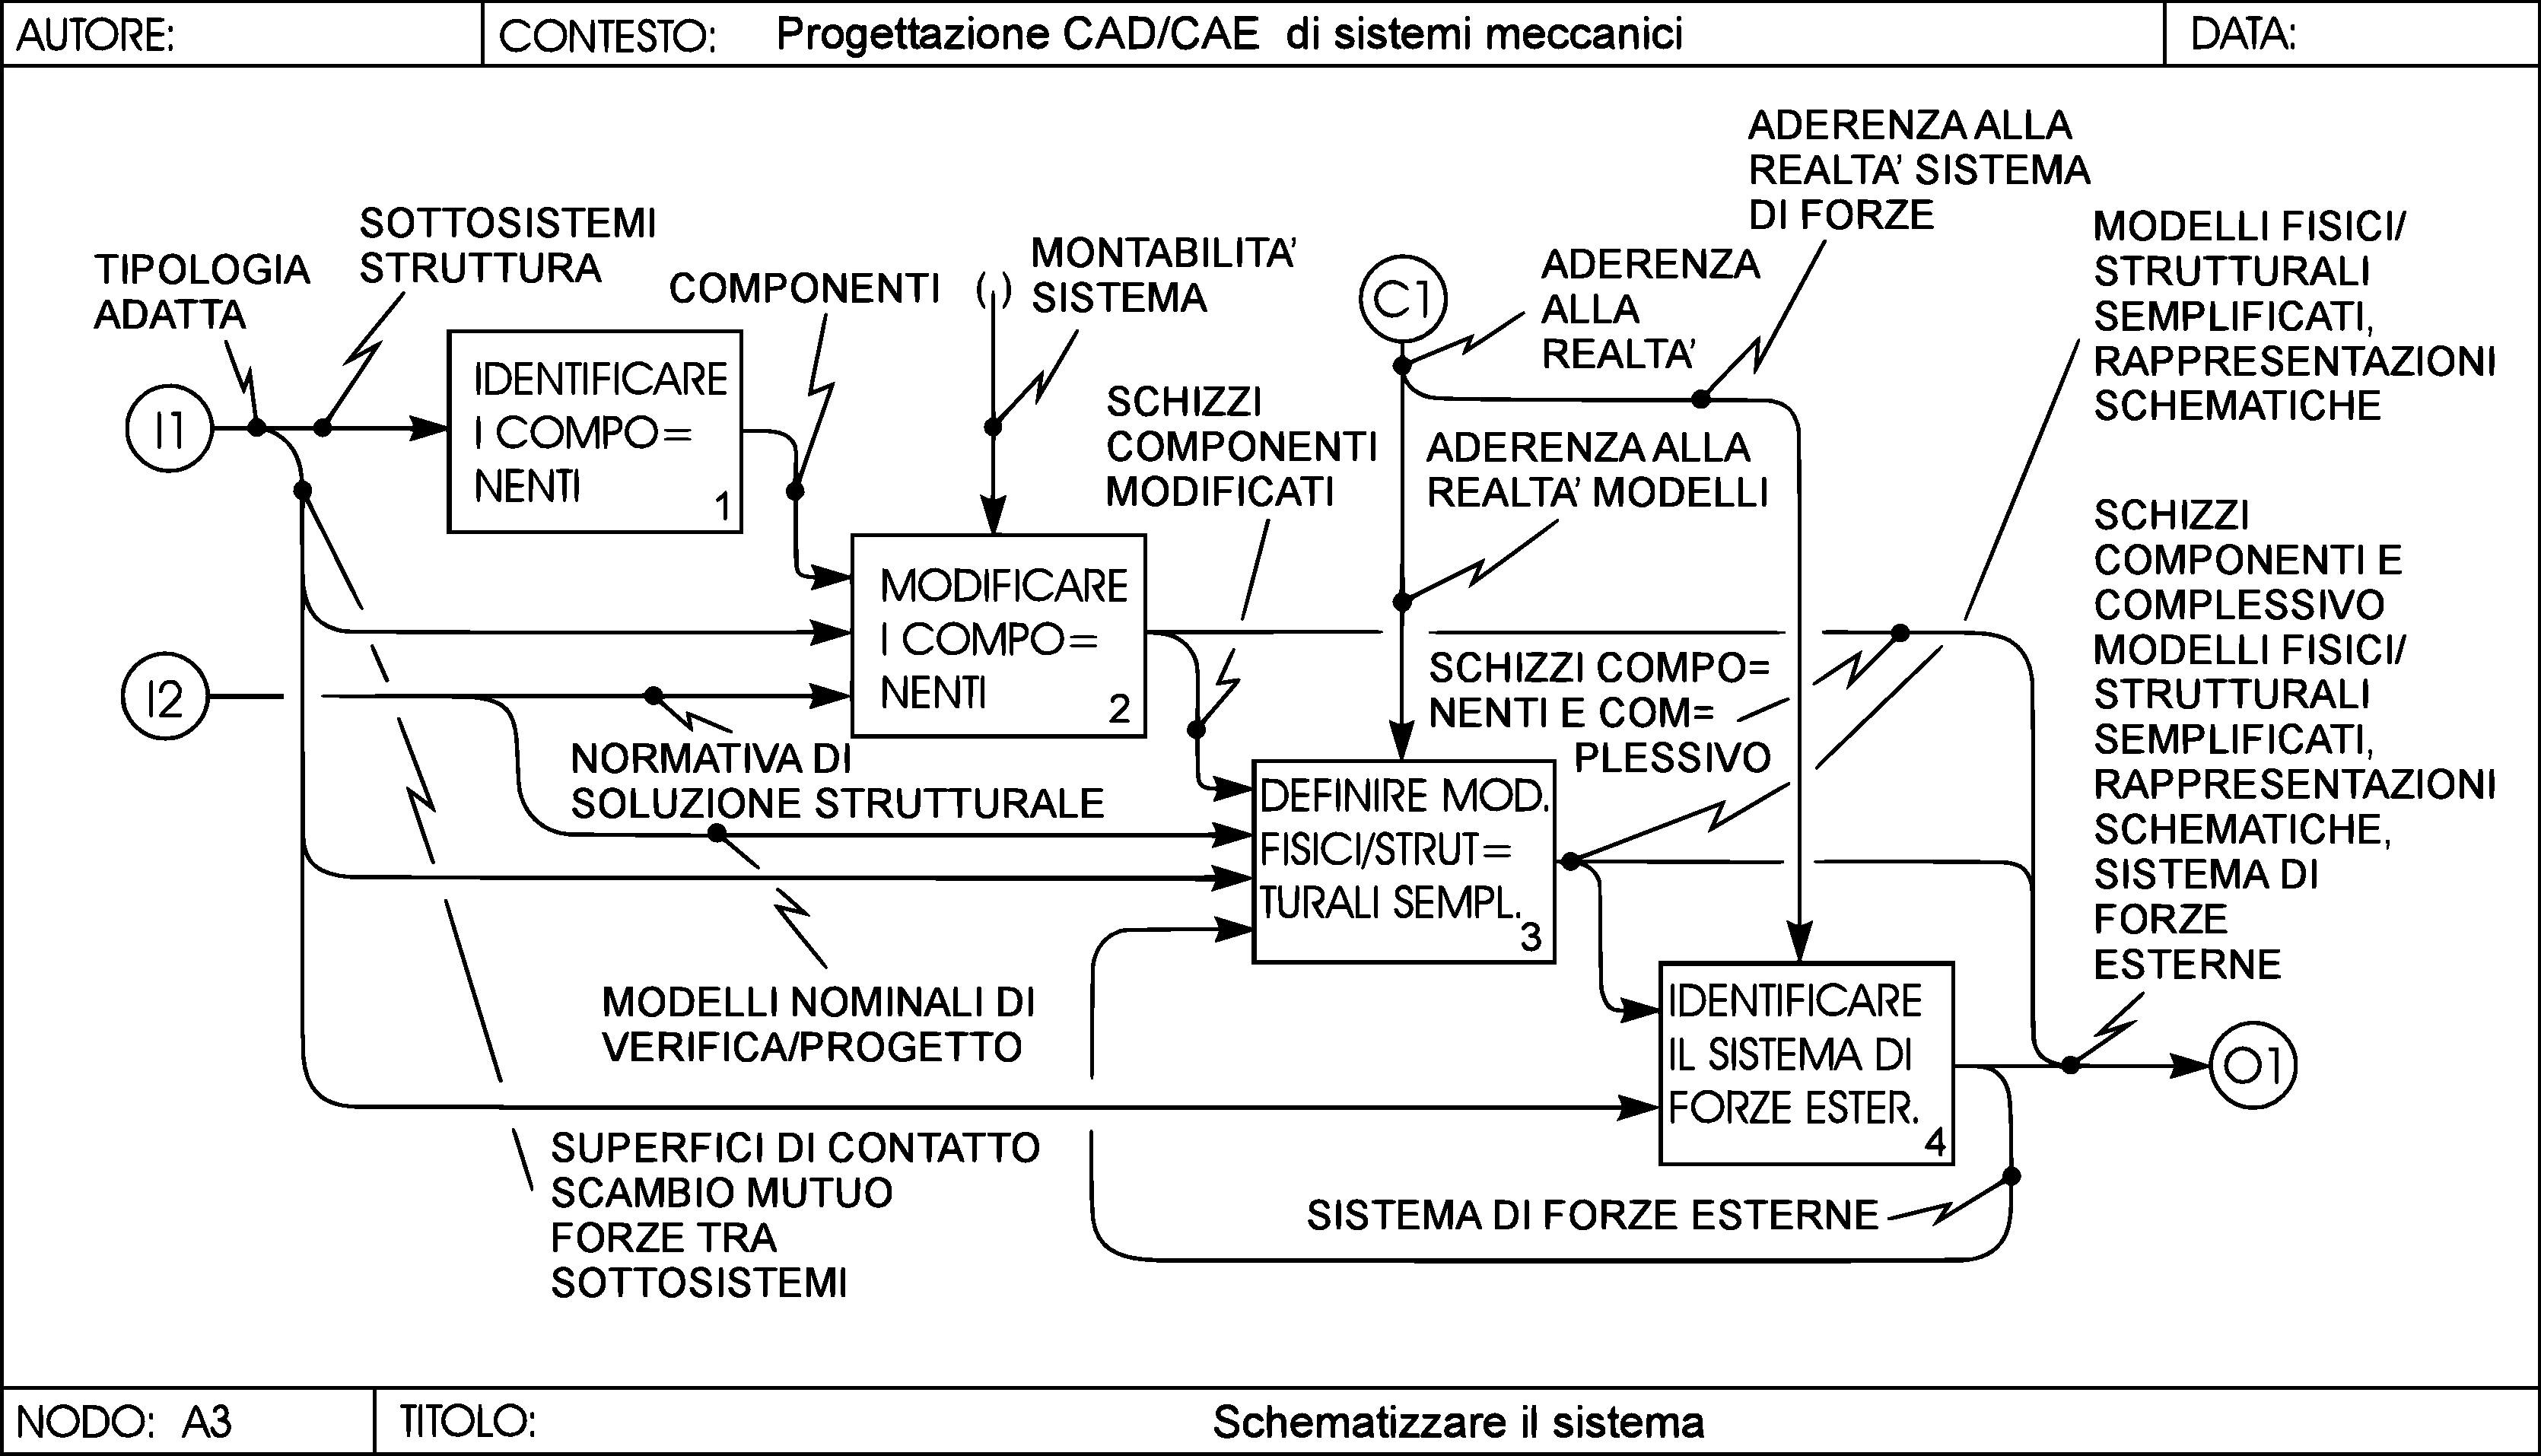
\includegraphics[width=.6\textwidth]{imgs/NodoA3.pdf}
\caption{Nodo A3}
\label{fig:NodoA3}
\end{figure}
Il nodo A3 consiste nella schematizzazione del sistema in esame. All'interno vengono individuati i blocchi relativi ai diversi componenti e alla loro modifica, alla definizione dei modelli fisici strutturali semplificati utilizzati nell'analisi e le forze agenti sullo stesso. In input vi sono i componenti stessi, in output si hanno gli schizzi dei componenti modificati. Definiti i modelli fisici utilizzati nello studio del sistema, si vanno a stabilire le forze agenti sul modello e le conseguenti sollecitazioni. 

Gli input I1 effettivi consistono nella forma di
\begin{itemize}
\item Gancio;
\item Traversa;
\item Bozzello scatolato o con lamoni e piastroni;
\item Numero e forma delle pulegge.
\end{itemize}
All'interno del blocco "modifica dei componenti" sono presenti riferimenti alle normative per sistemi di sollevamento e un controllo relativo alla montabilità del sistema. 
Vengono poi inseriti dei blocchi relativi all'aderenza alla realtà dei modelli fisici utilizzati e del sistema di forze agenti sul sistema.
Il blocco relativo ai modelli fisici semplificati individua nuovi input I2 non presenti nel livello superiore.
L'output del blocco 3 comprende:
\begin{itemize}
\item Modelli fisici semplificati;
\item Schizzi dei componenti;
\item Rappresentazioni schematiche;
\item Sistemi di forze esterne.
\end{itemize}
Risutla chiaro che tutti questi elementi debbano trovarsi nell'output finale O1 del diagramma A3 in quanto sono anche input del blocco 4. 

\subsection{Nodo A4}
\begin{figure}[h!]
\centering
  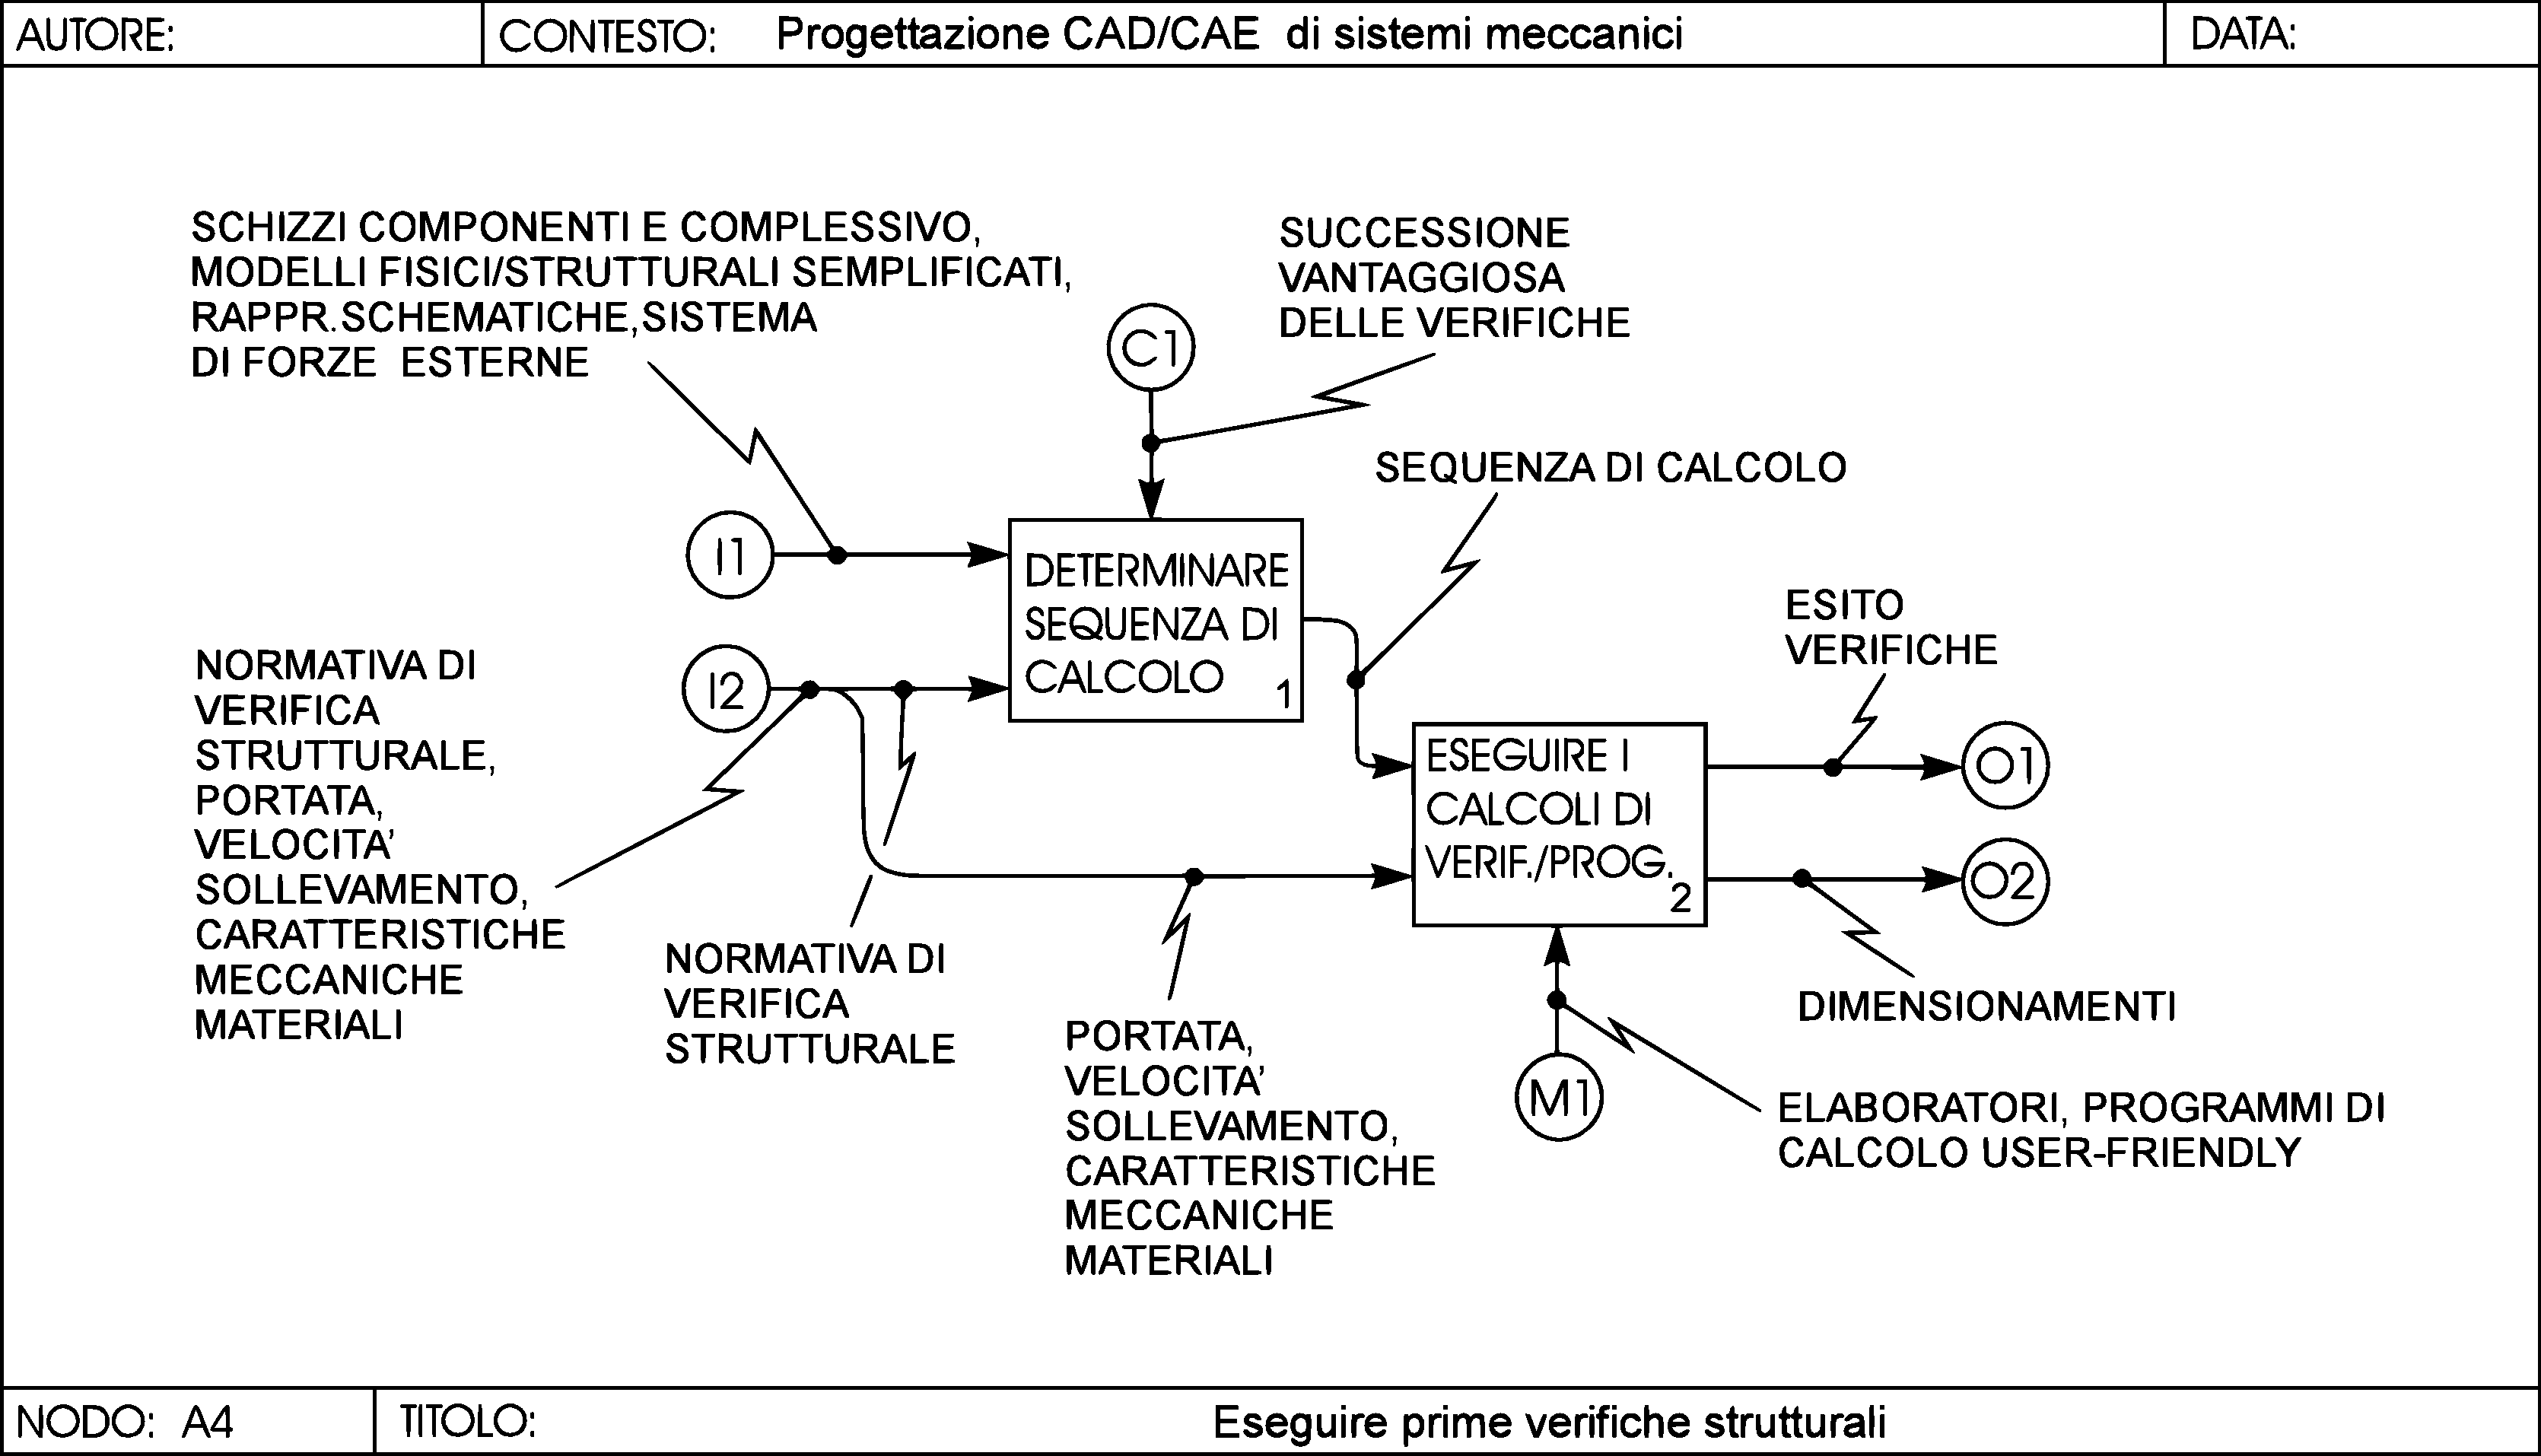
\includegraphics[width=.6\textwidth]{imgs/NodoA4.pdf}
\caption{Nodo A4}
\label{fig:NodoA4}
\end{figure}
Il nodo A4 riguarda le verifiche strutturali preliminari.
In questo contesto nel blocco 1 si determina la sequanza di calcolo con gli input precedentemente definiti.
L'output prodotto consiste semplicemente nell'ordine di verifica che viene utilizzata nel nodo 2 (calcoli di verifica). 
Con l'esito delle verifiche si determina un feed-back di controllo che può portare a successive modifiche delle soluzioni progettuali.
Ultimo ma non meno importante, come input per le diverse verifiche ci sono naturalmente portata del gancio, velocità di sollevamento e le caratteristiche meccaniche dei materiali.

\subsection{Nodo A5}
\begin{figure}[h!]
\centering
  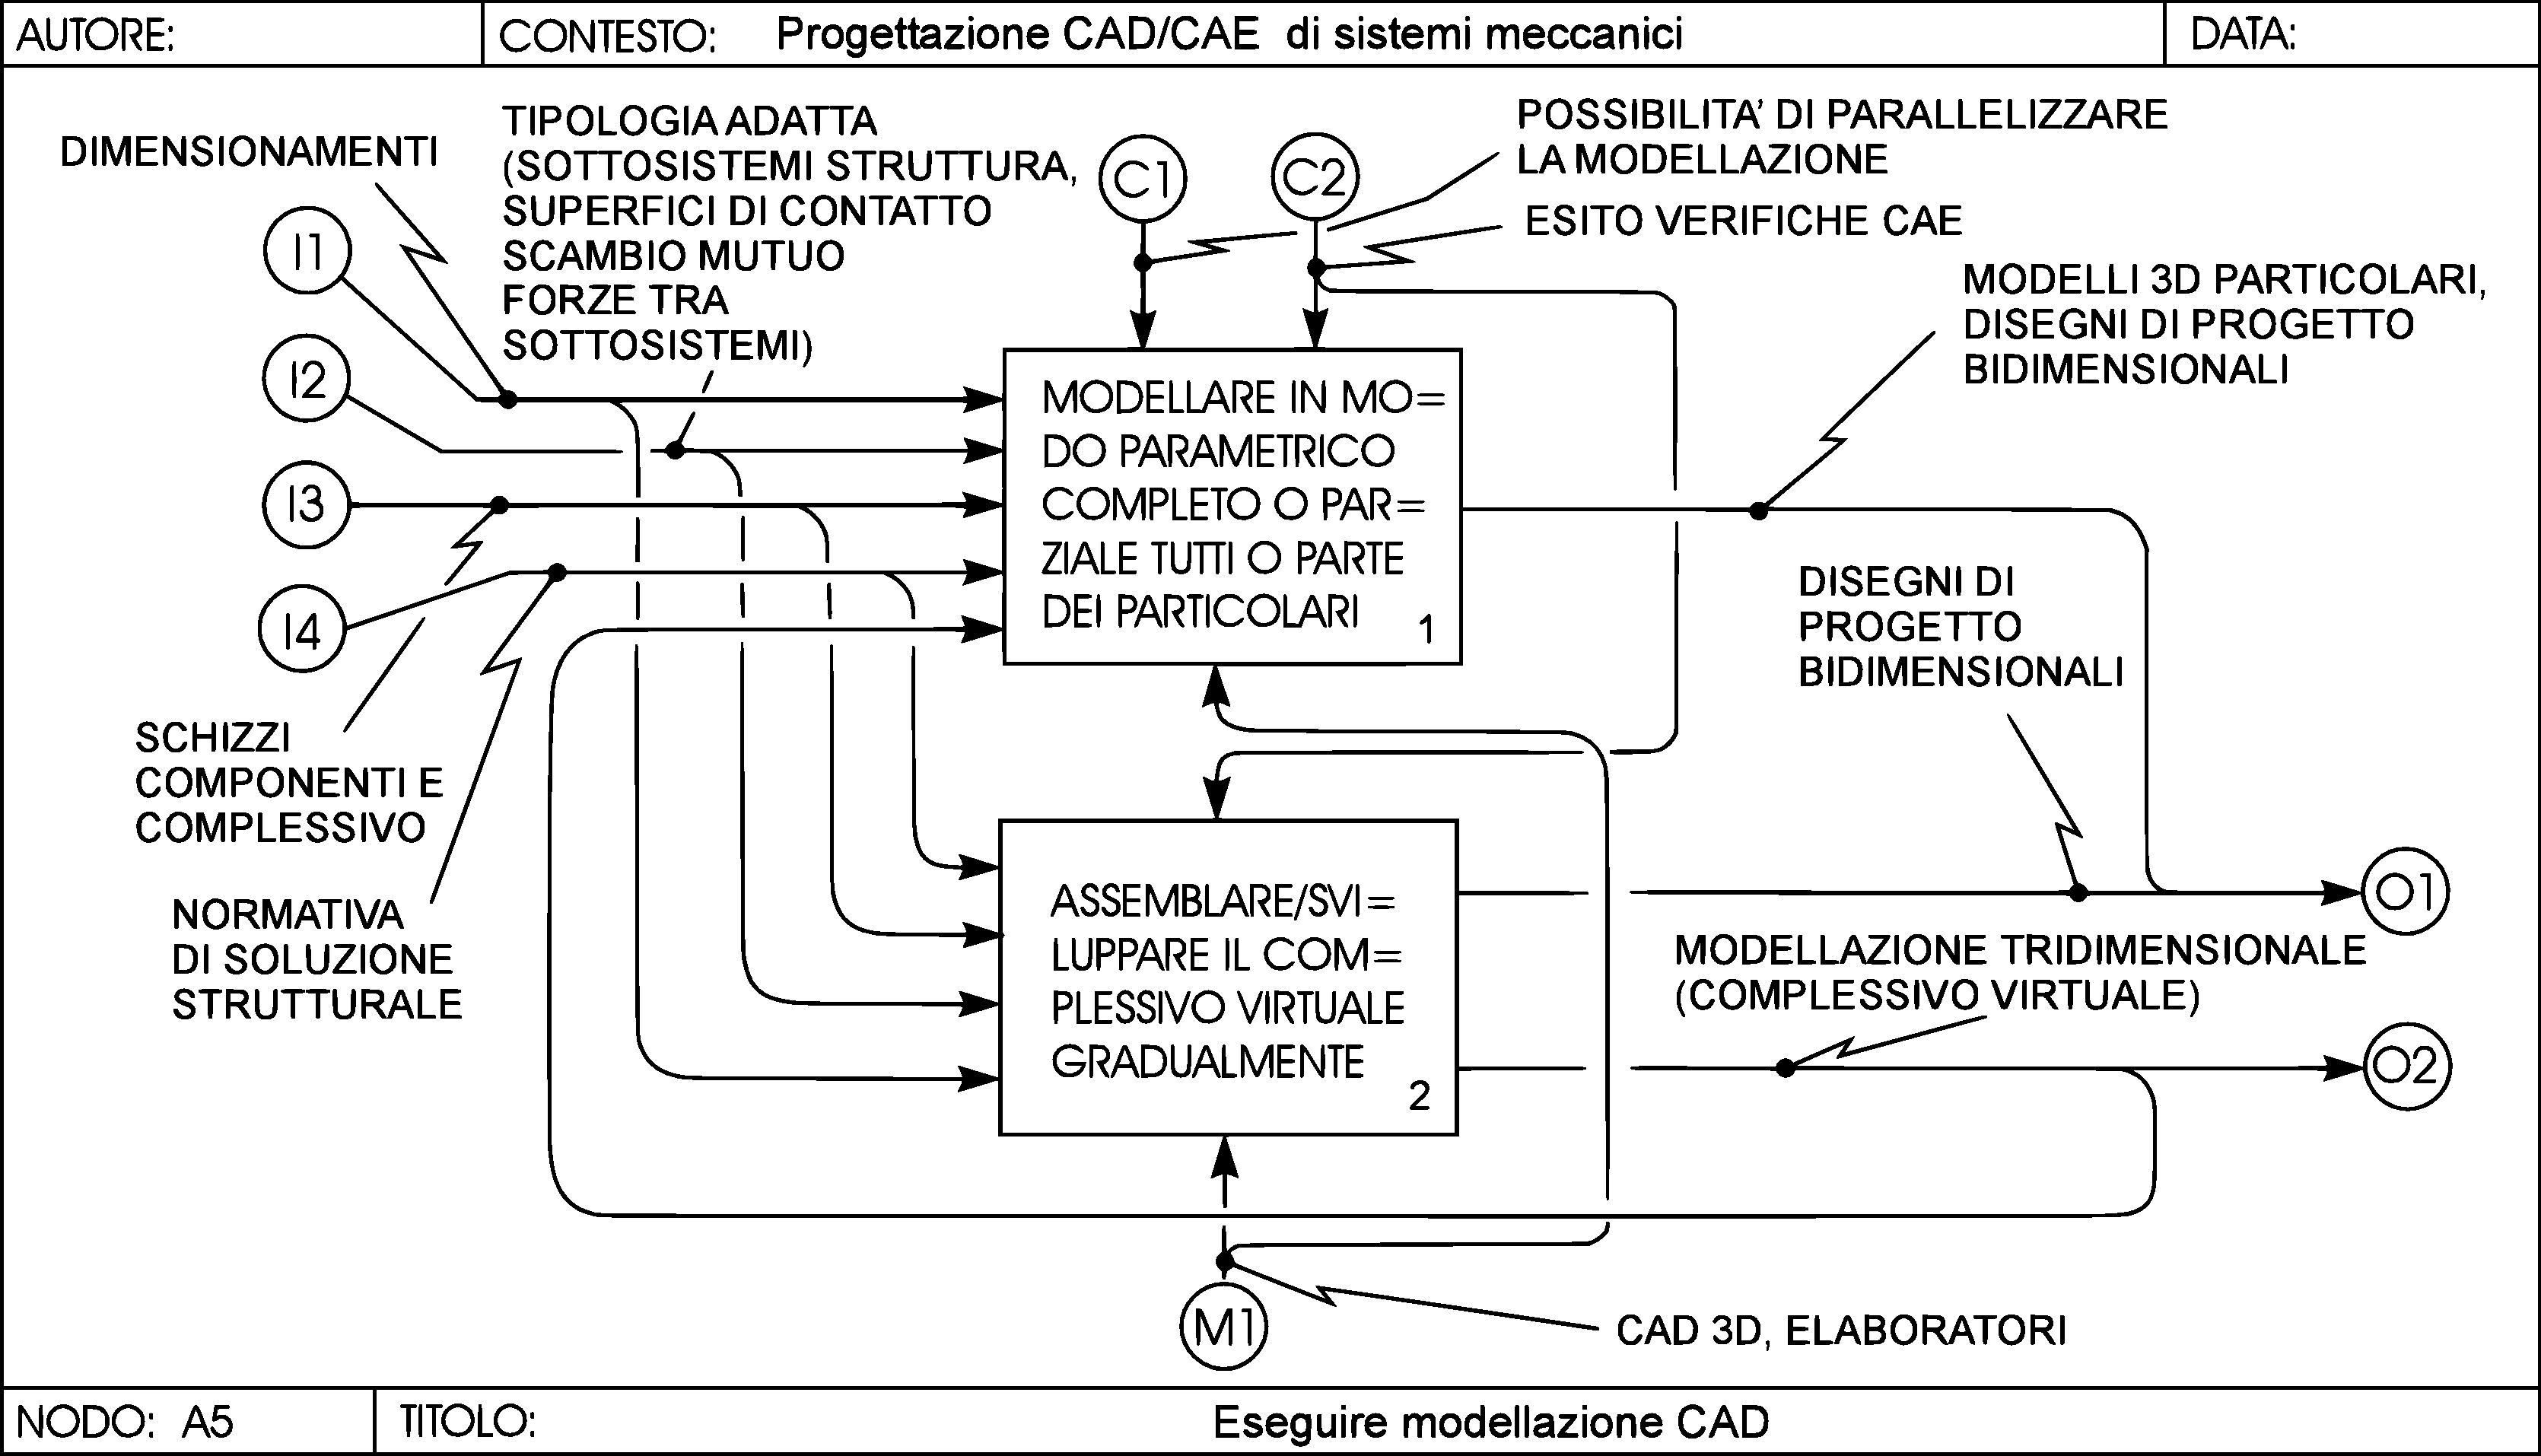
\includegraphics[width=.7\textwidth]{imgs/NodoA5.pdf}
\caption{Nodo A5}
\label{fig:NodoA5}
\end{figure}
Il nodo A5 comprende la modellazione CAD del sistema. 
Gli input sono i seguenti:
\begin{itemize}
\item Dimensionamenti preliminari;
\item Schizzi dei componenti e del complessivo;
\item Tipologia;
\item Normativa di soluzione strutturale.
\end{itemize}
L'output consiste naturalmente nei disegni di progetto bidimensionali e nel modello tridimensionale. Dalla figura \ref{fig:NodoA5} si nota che non è presente dominanza funzionale tra i blocchi 1 e 2, la disposizione è in fatti incolonnata e non diagonale. 

\subsection{Nodo A6}
\begin{figure}[h!]
\centering
  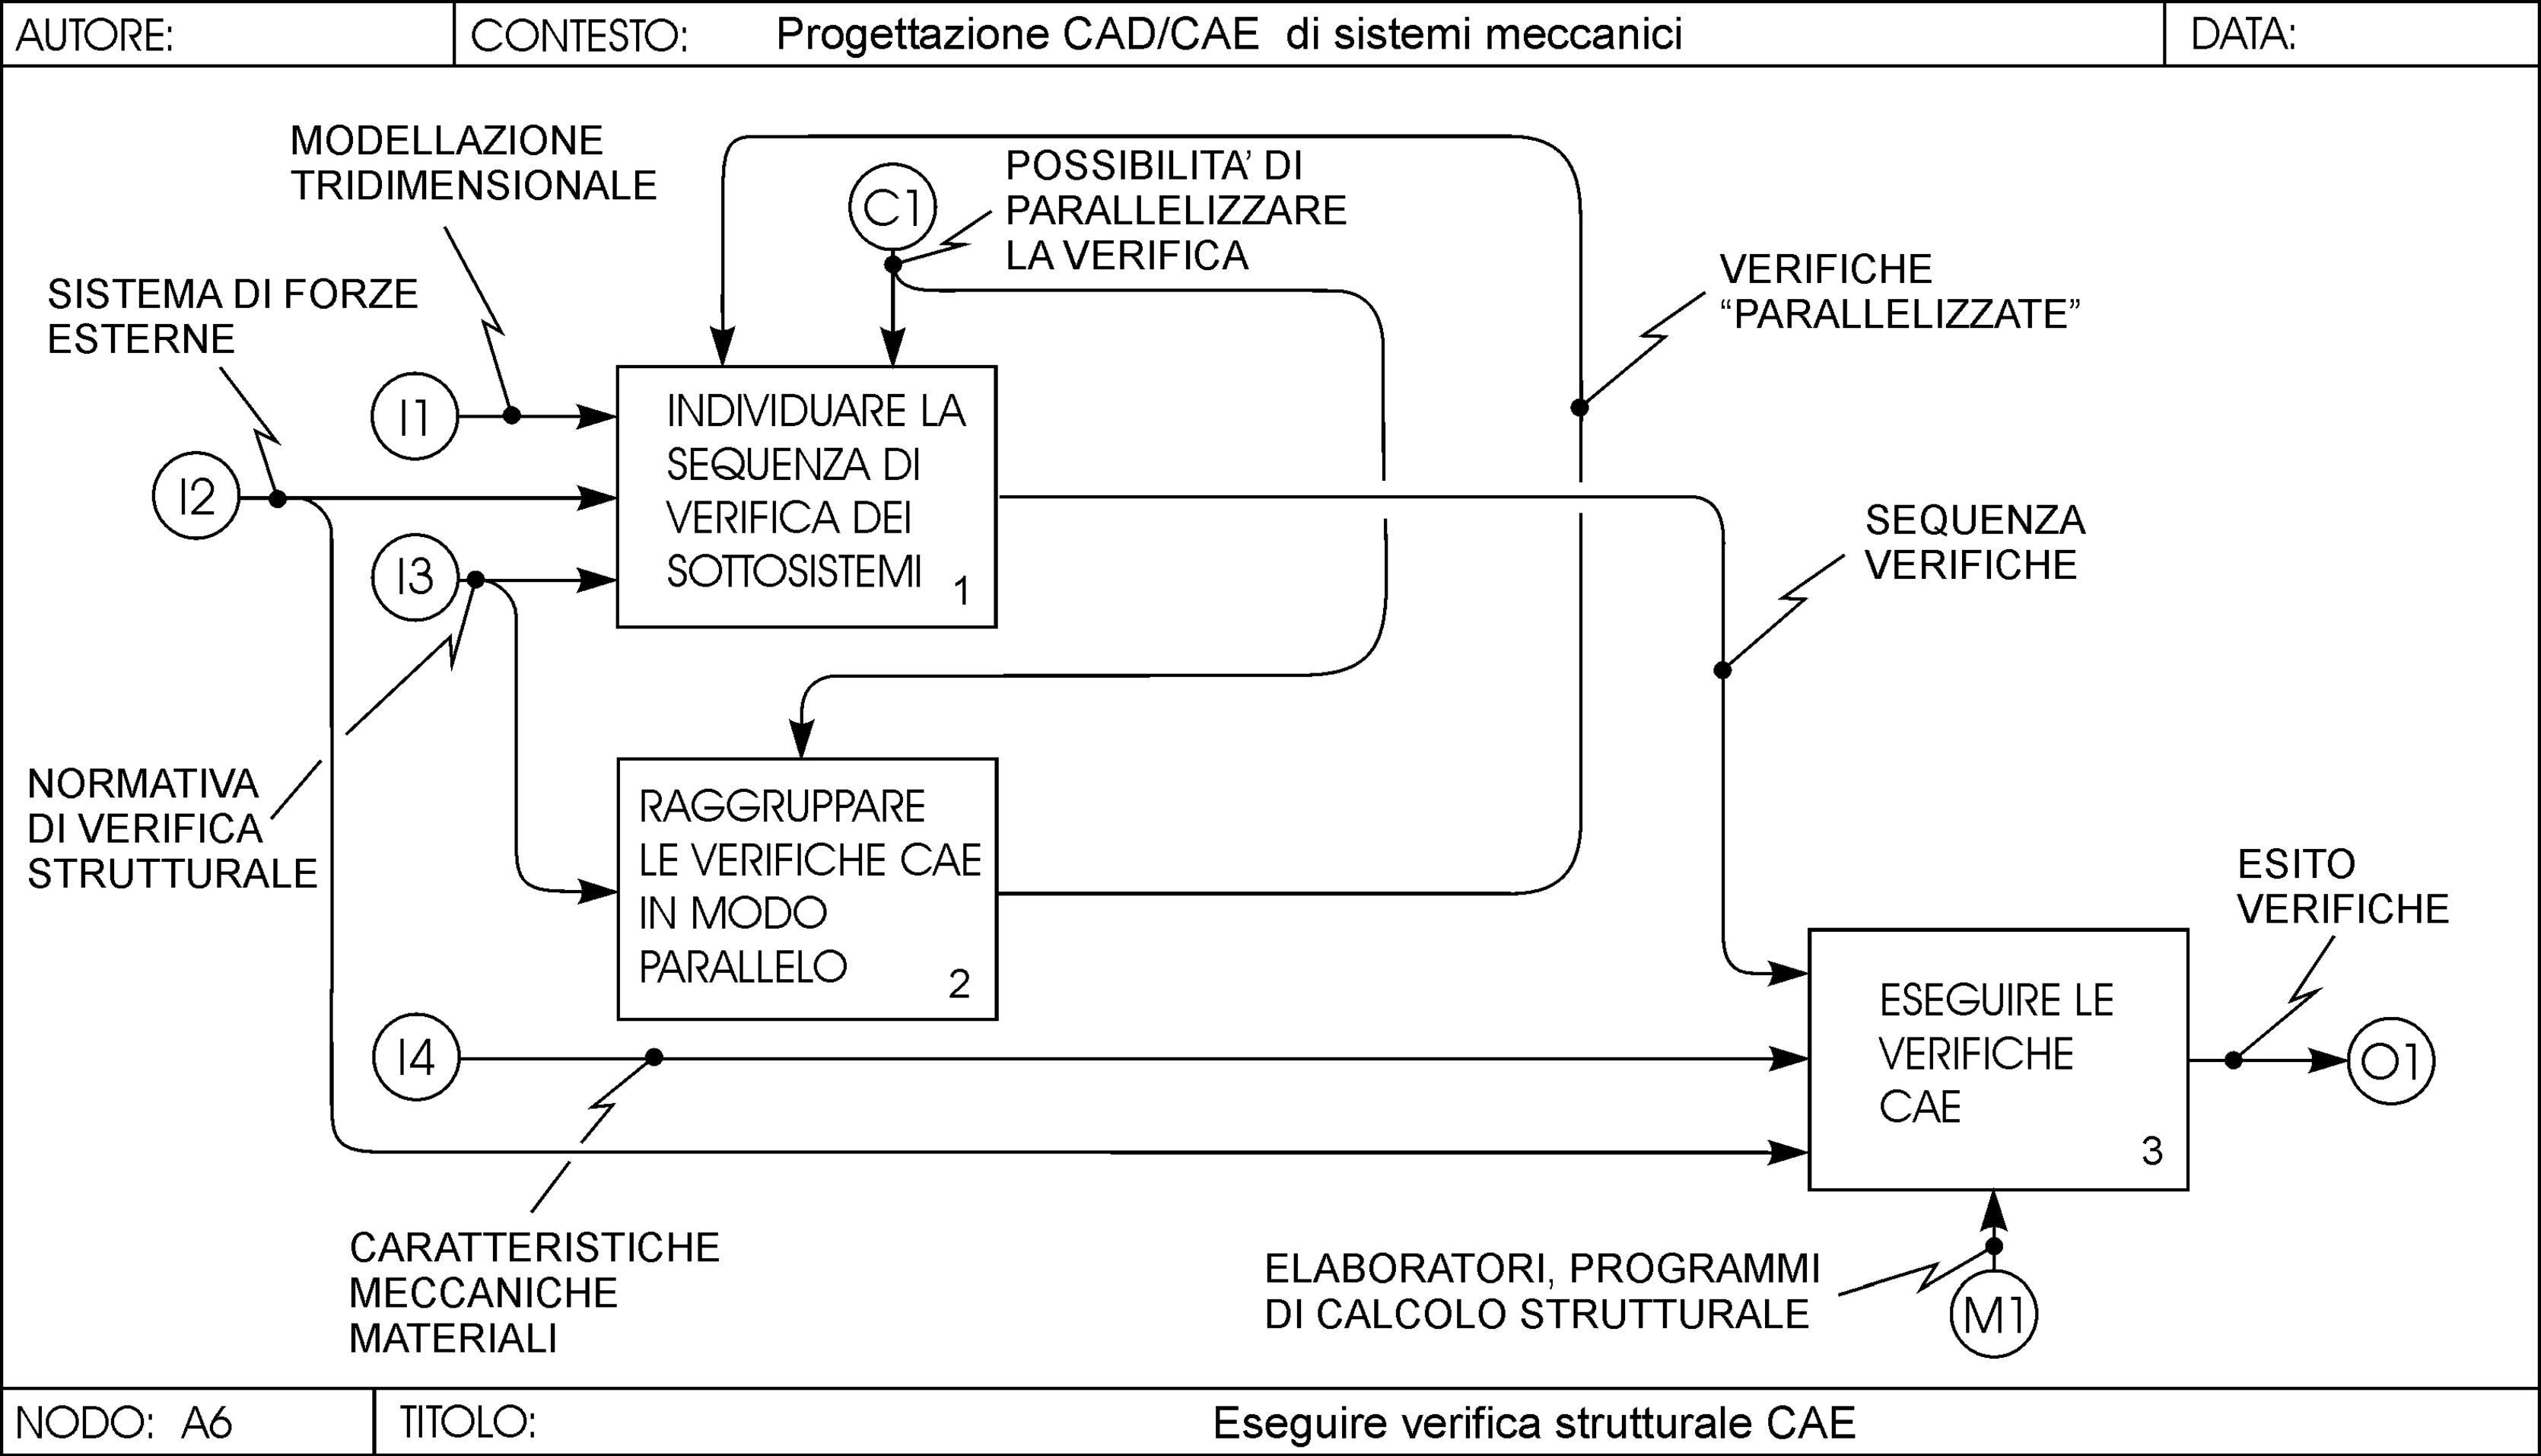
\includegraphics[width=.6\textwidth]{imgs/NodoA6.pdf}
\caption{Nodo A6}
\label{fig:NodoA6}
\end{figure}
Nel nodo A6 sono presenti le verifiche strutturali. Dalla figura \ref{fig:NodoA6} si può vedere la presenza di tre blocchi, nel primo si determina la sequenza di verifica dei sottoinsiemi, il secondo determina le verifiche che sono parllelizzabili e nel terzo si eseguono effettivamente tali verifiche.
I controlli riguardano invece l'impiego dei software utilizzati.
Come input sono previsti il sistema di forze esterne, il modello 3D e la normativa di verifica strutturale che fornisce le procedure di verifica al fine di aumentare la sicurezza del sistema.

\subsection{Nodo A33}
\begin{figure}[h!]
\centering
  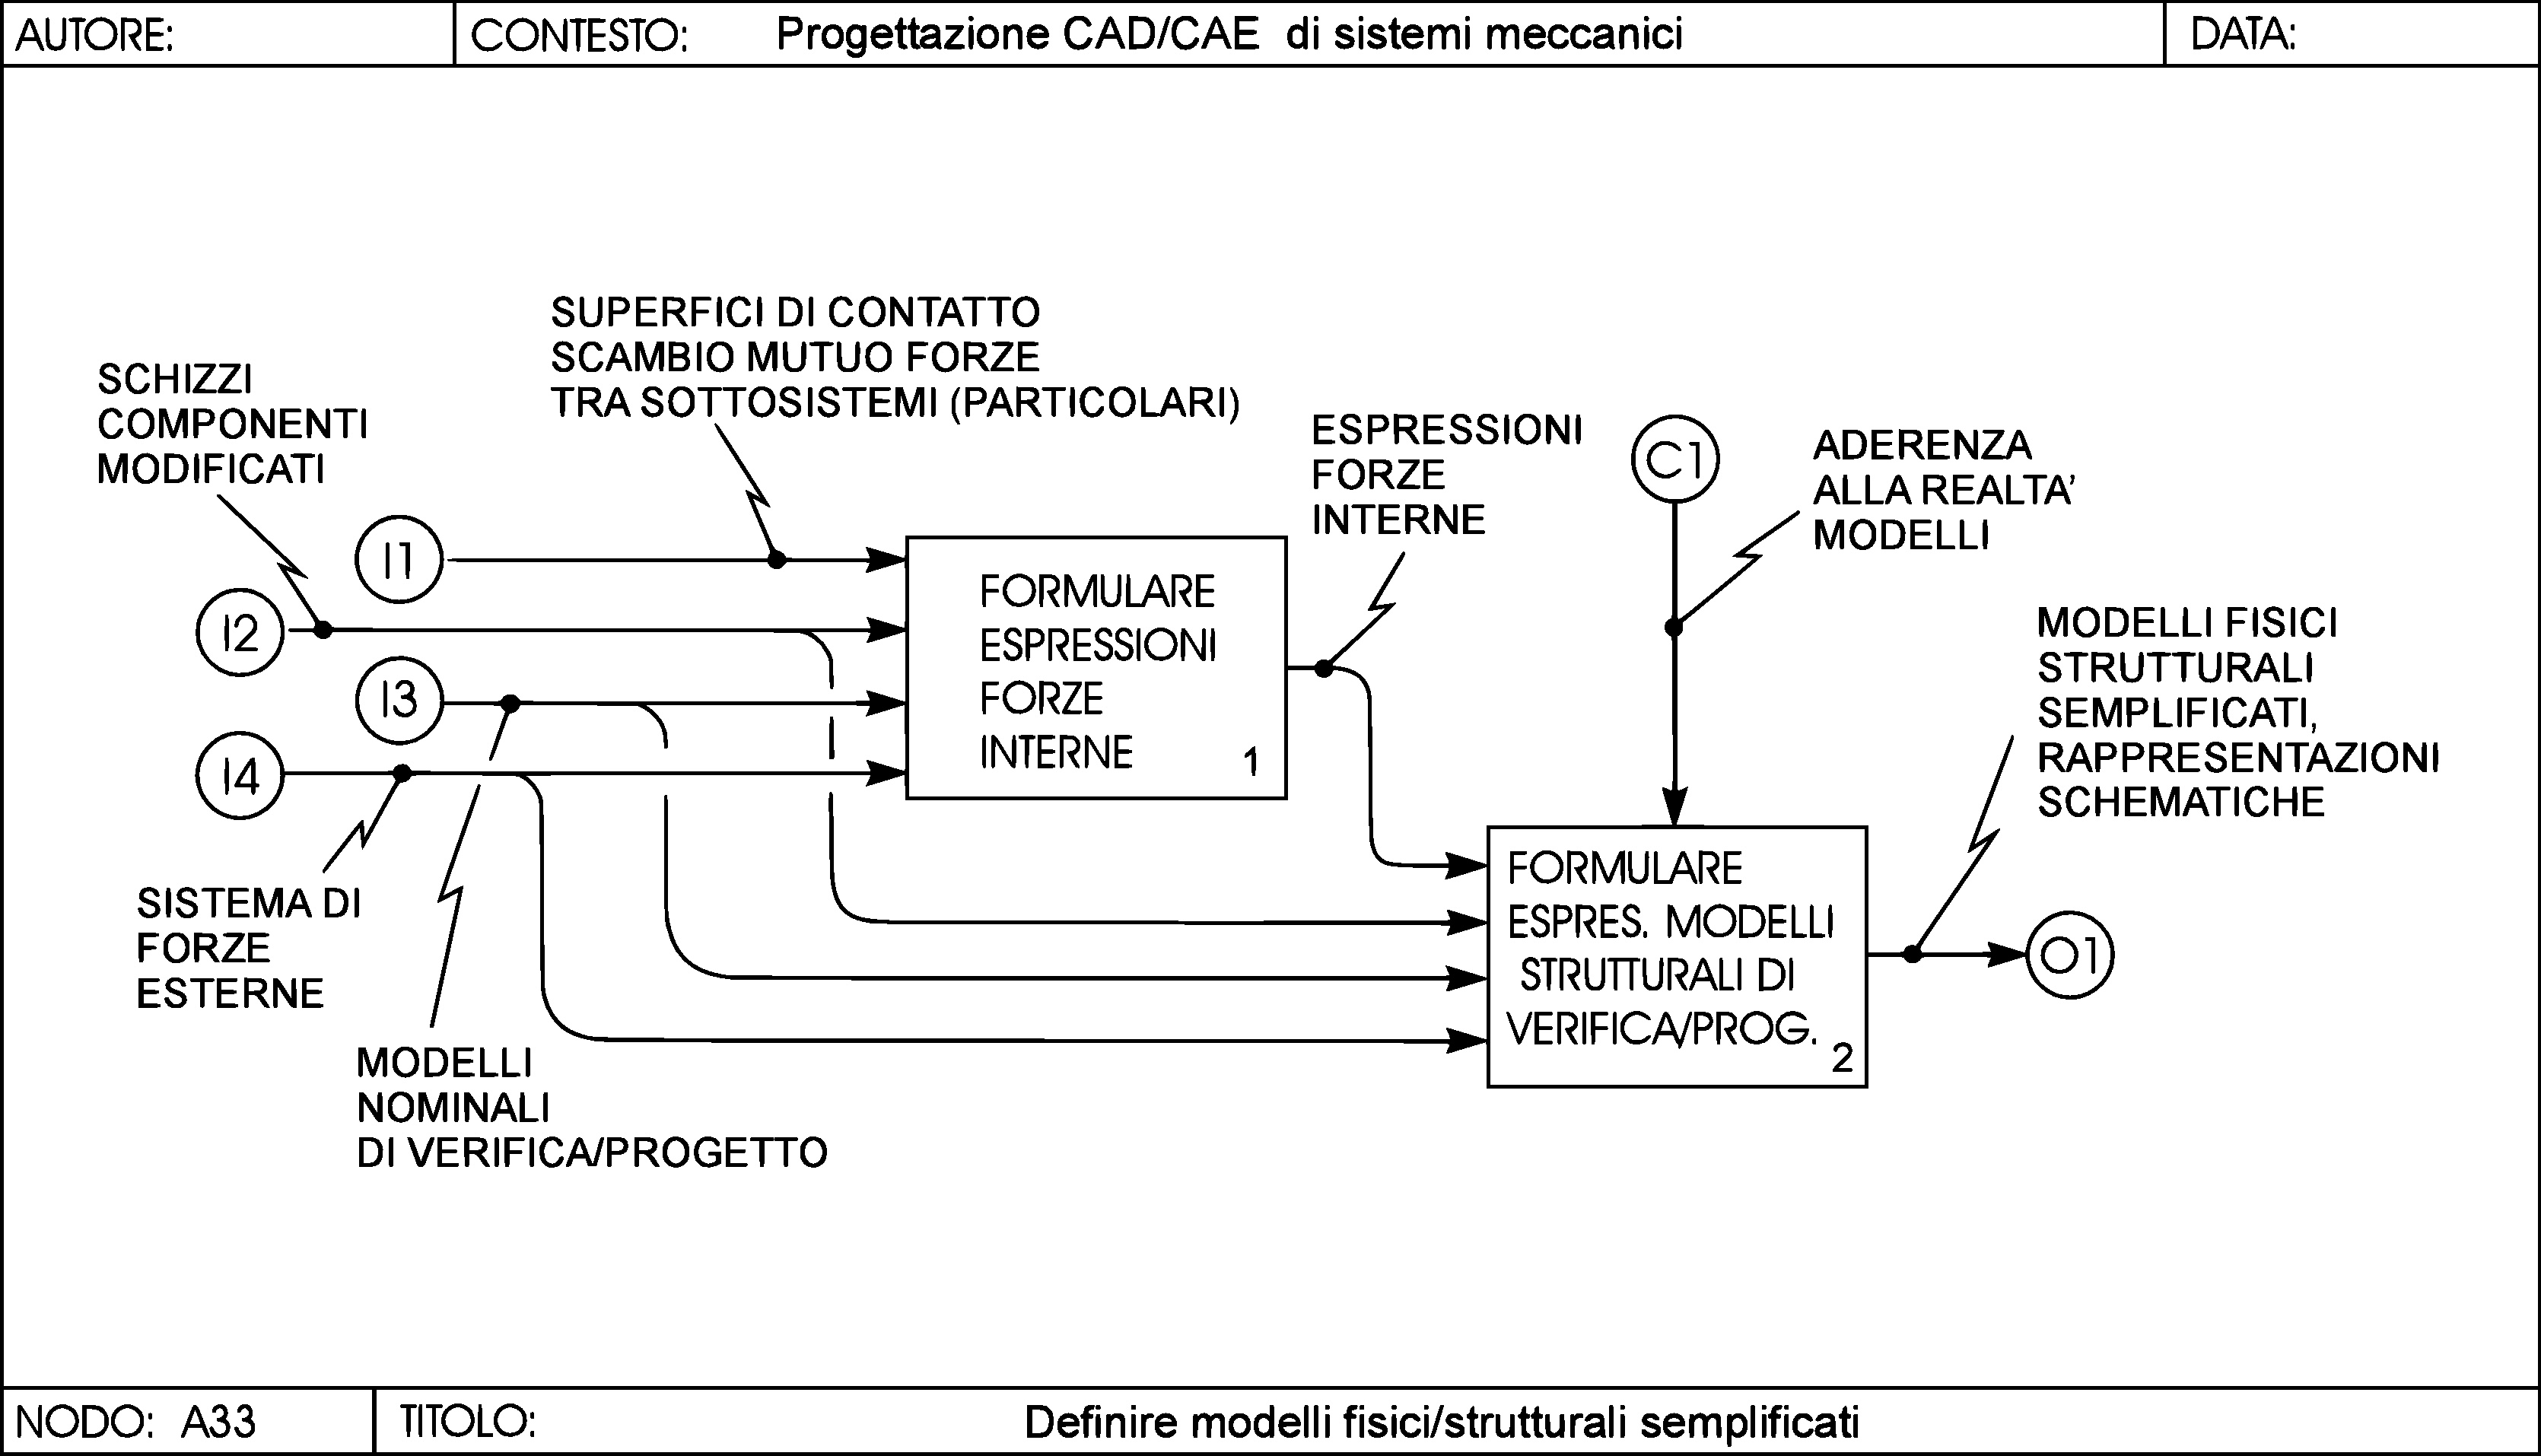
\includegraphics[width=.6\textwidth]{imgs/NodoA33.pdf}
\caption{Nodo A33}
\label{fig:NodoA33}
\end{figure}
A questo punto possiamo vedere che l'attività "Progettazione CAD/CAE di sistemi meccanici" del nodo A3 può essere scomposta in due ulteriori blocchi: formulazione delle espressioni delle forze internee formulazione di espressioni e modelli strutturali di verifica e progetto.

L'analisi SADT è stata fondamentale per ridurre i gradi di liberà di progettaizione e definire le attività in maniera chiara. 